\documentclass[border=10pt]{standalone}
\usepackage{tkz-fct}
\usepackage{tkz-base}
\usepackage{array}

\begin{document}

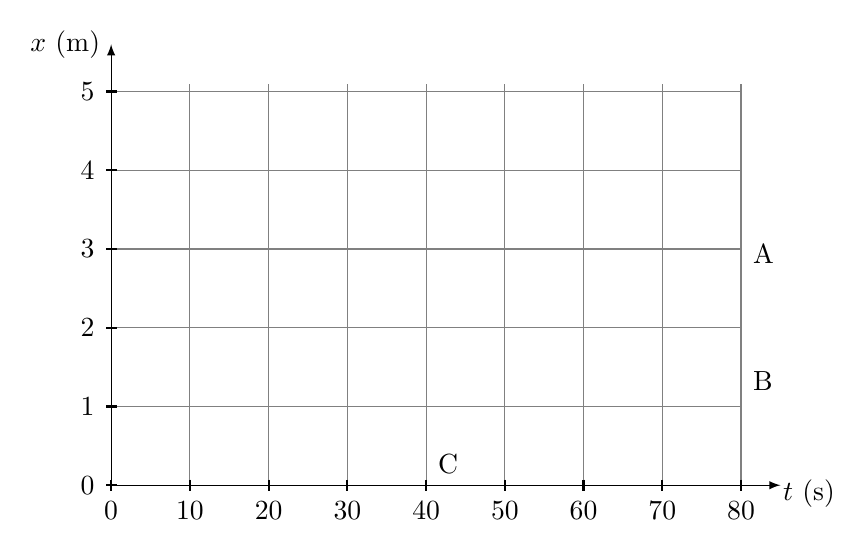
\begin{tikzpicture}
% Tableau en LaTeX standard avec tkz-text

% Repère quadrillé
\tkzInit[xmin=0,xmax=80,xstep=10,ymin=0,ymax=5.1, ystep=1]
\tkzGrid
\tkzDrawX[label = $t$ (s), right]
\tkzDrawY[label = $x$ (m)]
\tkzLabelXY
\tkzFct[line width=2pt, domain=0:80]{(2/60.)*\x}
\tkzDefPointByFct(80)
\tkzText[above right](tkzPointResult){A}
\tkzFct[line width=2pt, domain=0:80]{(-1/10.)*\x+4}
\tkzDefPointByFct(40)
\tkzText[above right](tkzPointResult){C}

\tkzFct[line width=2pt, domain=0:80]{(-1/50.)*(\x-10)+3}
\tkzDefPointByFct(80)
\tkzText[below right](tkzPointResult){B}

\end{tikzpicture}

\end{document}
